
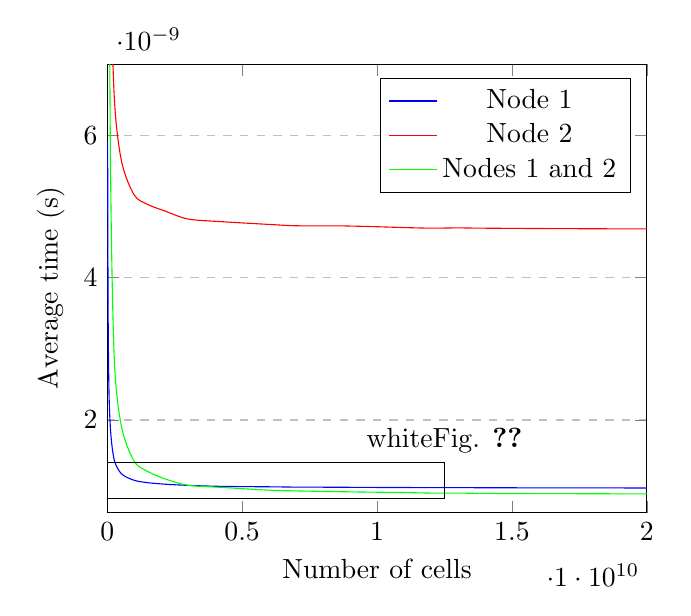
\begin{tikzpicture}
\begin{axis}[
    %title={Average time per cell},
    xlabel={Number of cells},
    ylabel={Average time (s)},
    xmin=0, xmax=20000000000,
    ymin=7e-10, ymax=7e-09,
    legend pos=north east,
    ymajorgrids=true,
    grid style=dashed,
    scaled x ticks={real:10000000000},
]


\addplot[
    color=blue,
    smooth,
    ]
    coordinates {
    (16777216, 5.9137855257306775e-09)(33554432, 3.600158861705235e-09)(67108864, 2.3944228887557983e-09)(134217728, 1.8066061394555226e-09)(268435456, 1.4282848153795516e-09)(536870912, 1.2414301080363135e-09)(1000000000, 1.152977142857143e-09)(1500000000, 1.119065714285714e-09)(2147483648, 1.0979907321078438e-09)(3000000000, 1.0814785714285714e-09)(4294967296, 1.0668948691870486e-09)(6000000000, 1.0614280952380955e-09)(7000000000, 1.057224693877551e-09)(8589934592, 1.0550598381087185e-09)(10000000000, 1.0521971428571429e-09)(11000000000, 1.0512831168831168e-09)(12000000000, 1.0494261904761902e-09)(13000000000, 1.0495164835164835e-09)(14000000000, 1.0483724489795918e-09)(17179869184, 1.0460199389074528e-09)(25769803776, 1.0433235383104711e-09)(34359738368, 1.042618532665074e-09)(42949672960, 1.0408397897013597e-09)(51539607552, 1.0398679435075748e-09)(60129542144, 1.0400224115927607e-09)(68719476736, 1.0391142235935798e-09)(77309411328, 1.0390710529117357e-09)(85899345920, 1.0391409575406993e-09)(94489280512, 1.0389721250863041e-09)(100000000000, 1.0383371428571429e-09)(103079215104, 1.0382666784737793e-09)(111669149696, 1.038346634051957e-09)(120259084288, 1.0378354666184407e-09)
    };

\addplot[
    color=red,
    smooth,
    ]
    coordinates {
    (16777216, 3.245565720966884e-08)(33554432, 1.8672138452529907e-08)(67108864, 1.1961538876805988e-08)(134217728, 8.379966020584107e-09)(268435456, 6.4965124641145975e-09)(536870912, 5.626971168177468e-09)(1000000000, 5.162437142857143e-09)(1500000000, 5.029282857142857e-09)(2147483648, 4.935963079333305e-09)(3000000000, 4.824004761904761e-09)(4294967296, 4.785867141825813e-09)(6000000000, 4.748461904761905e-09)(7000000000, 4.729608163265305e-09)(8589934592, 4.728251535977636e-09)(10000000000, 4.7160128571428574e-09)(11000000000, 4.704388311688311e-09)(12000000000, 4.696046428571429e-09)(13000000000, 4.699453846153845e-09)(14000000000, 4.695503061224491e-09)(17179869184, 4.688792562644397e-09)(25769803776, 4.678011117946534e-09)(34359738368, 4.6729318065834904e-09)(42949672960, 4.667090252041816e-09)(51539607552, 4.665895609096402e-09)(60129542144, 4.661319378231253e-09)(68719476736, 4.661219593669687e-09)(77309411328, 4.661910694151644e-09)(85899345920, 4.659480016146388e-09)(94489280512, 4.6594083526885355e-09)(100000000000, 4.6598900000000005e-09)(103079215104, 4.659376351074094e-09)(111669149696, 4.6597087530644385e-09)(120259084288, 4.659140748637063e-09)
    };

\addplot[
    color=green,
    smooth,
    ]
    coordinates {
    (16777216, 2.9583752155303957e-08)(33554432, 1.514038017817906e-08)(67108864, 9.290228996958051e-09)(134217728, 5.197258932249886e-09)(268435456, 2.8187840112618036e-09)(536870912, 1.8953390951667517e-09)(1000000000, 1.4202885714285714e-09)(1500000000, 1.277607619047619e-09)(2147483648, 1.1723881055201802e-09)(3000000000, 1.083004761904762e-09)(4294967296, 1.0516730669353688e-09)(6000000000, 1.0138707142857144e-09)(7000000000, 1.003642244897959e-09)(8589934592, 9.929328225553036e-10)(10000000000, 9.85383e-10)(11000000000, 9.808103896103896e-10)(12000000000, 9.733238095238094e-10)(13000000000, 9.729956043956044e-10)(14000000000, 9.68534693877551e-10)(17179869184, 9.647562235061612e-10)(25769803776, 9.547974470825421e-10)(34359738368, 9.519322442689111e-10)(42949672960, 9.487150236964226e-10)(51539607552, 9.463479121526082e-10)(60129542144, 9.423898704045889e-10)(68719476736, 9.409590607642063e-10)(77309411328, 9.429238234010953e-10)(85899345920, 9.43106466106006e-10)(94489280512, 9.422190487384794e-10)(100000000000, 9.425682857142859e-10)(103079215104, 9.416450103301378e-10)(111669149696, 9.416758625225706e-10)(120259084288, 9.41362802167328e-10)
    };

\addplot[
    color=black,
    mark=none,
] coordinates {(0,9e-10) (0,1.4e-09) (12500000000,1.4e-09) (12500000000,9e-10) (0,9e-10)};

\pgfplotsset{
    after end axis/.code={
        \node[above] at (axis cs:12500000000,1.4e-09){\contour{white}{Fig. \ref{result_graph_cell_zoom}}};
    }
}


\legend{Node 1, Node 2, Nodes 1 and 2}
\end{axis}
\end{tikzpicture}
